% Octeto barionico de spin 1/2: diagrama de peso SU(3) (Y vs I_3) — libro fig. 7.3
\documentclass[border=5pt]{standalone}
\usepackage{amsmath}
\usepackage{tikz}
\usetikzlibrary{arrows.meta, calc}
\begin{document}
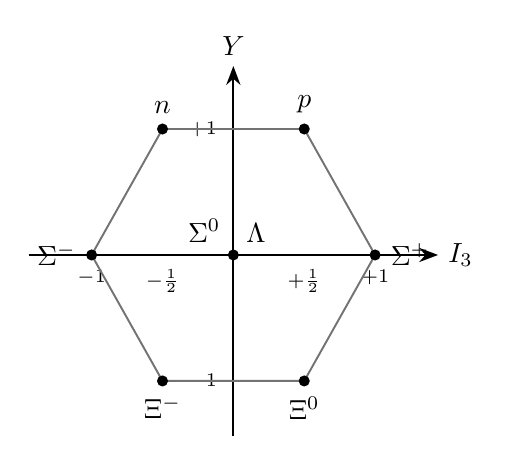
\begin{tikzpicture}[>={Stealth[length=2.4mm]}, line width=0.7pt]
  % ejes
  \draw[->] (-2.6,0)--(2.6,0) node[right]{$I_3$};
  \draw[->] (0,-2.3)--(0,2.4) node[above]{$Y$};
  \foreach \x/\l in {-1.8/-1,-0.9/-\tfrac12,0.9/+\tfrac12,1.8/+1}{\node[below, font=\scriptsize] at (\x,-0.06){$\l$};}
  \node[left, font=\scriptsize] at (-0.08,1.6){$+1$};
  \node[left, font=\scriptsize] at (-0.08,-1.6){$-1$};
  % posiciones de las 8 particulas
  \coordinate (n) at (-0.9,1.6);  \coordinate (p) at (0.9,1.6);
  \coordinate (Sm) at (-1.8,0);   \coordinate (S0) at (0,0);   \coordinate (Sp) at (1.8,0);
  \coordinate (Xm) at (-0.9,-1.6);\coordinate (X0) at (0.9,-1.6);
  % hexagono
  \draw[black!55] (n)--(p)--(Sp)--(X0)--(Xm)--(Sm)--cycle;
  % puntos + etiquetas
  \foreach \pt/\lab/\pos in {n/n/above,p/p/above,Sm/{\Sigma^-}/left,Sp/{\Sigma^+}/right,Xm/{\Xi^-}/below,X0/{\Xi^0}/below}{
    \fill (\pt) circle (2pt); \node[\pos=2pt] at (\pt){$\lab$};}
  % centro: Sigma0 y Lambda (dos particulas)
  \fill (S0) circle (2pt);
  \node[above left=1pt] at (S0){$\Sigma^0$};
  \node[above right=1pt] at (S0){$\Lambda$};
\end{tikzpicture}
\end{document}
